\section{Design and Implementation of \textsf{PCStream}}

\begin{figure}[t]
	\centering
	%\vspace{-10pt}
	%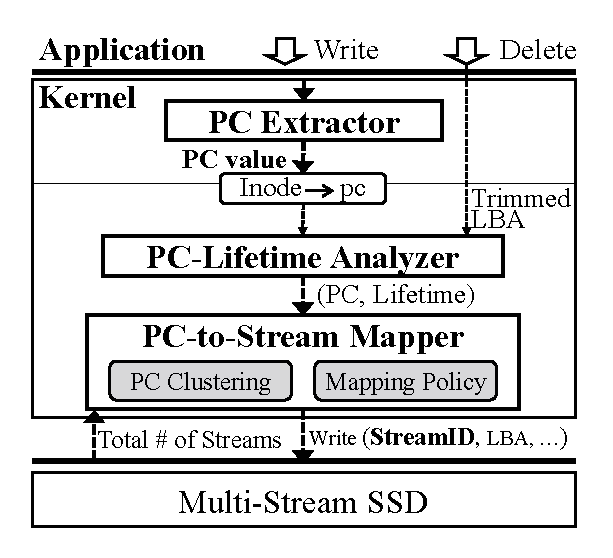
\includegraphics[width=0.6\linewidth]{figure/architecture4}
	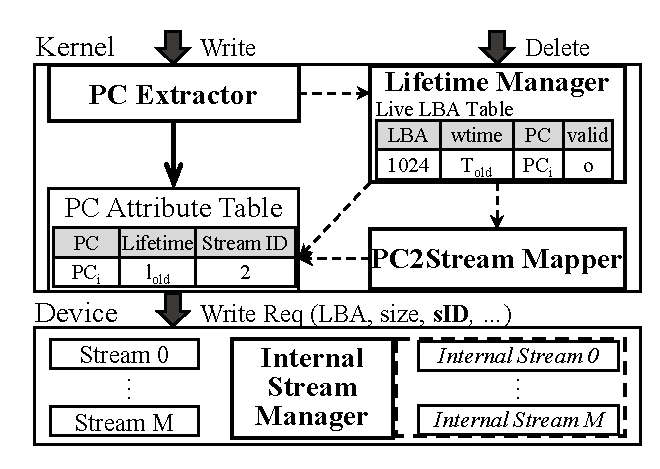
\includegraphics[width=0.6\linewidth]{figure/overview}
	%\vspace{-9pt}
	\caption{An overall architecture of \textsf{\small PCStream}.}
	\label{fig:architecture}
	%\vspace{-22pt}
\end{figure}

In this section, we explain the details of the proposed automatic stream
management technique, \textsf{\small PCStream}.
% COMMENT: maybe not necessary
%We first explain how we automatically extract PCs from applications at runtime
%and then describe how a large number of PCs are maintained in the DRAM memory
%and are mapped to a few streams available in an SSD.  Finally, we discuss
%design issues associated with the implementation of internal streams inside an
%SSD.
Fig.~\ref{fig:architecture} shows an overall organization of \textsf{\small
PCStream}. The \textit{PC extractor module} implemented as part of a system
call handler in the Linux kernel is responsible for computing \textit{a PC
signature},  A PC
signature is obtained by summing program counter values~\cite{PC} along the
execution path to write-related system calls (e.g., {\tt write()}).  With a PC
signature, data written through specific call paths of applications can be
monitored at the program context level.  A PC signature is then delivered to
the \textit{PC-lifetime manager}, which caches collected PC signatures in the
memory and estimates expected lifetimes of data belonging to given PCs.  Since
product SSDs only expose a limited number of streams outside, the
\textit{PC-stream cluster} groups PCs with similar lifetimes using a clustering 
policy. Data belonging to a same group have a same stream ID.

%the lifetime of data written by write-related system calls can be
%monitored at the program context level.  
%A PC signature value is stored in an
%inode data structure of a file system (modified for \textsf{\small PCStream})
%and is delivered to \textit{the lifetime analyzer module} which estimates
%expected lifetimes of data belonging to a given PC in the block device level.
%In order to efficiently detect the end of data lifetime in append-only
%workloads, the lifetime analyzer also intercepts TRIM~\cite{TRIM} requests from
%a file system.

%shane part Based on the lifetime information, \textit{the PC-to-stream mapper
%module} clusters PCs with similar lifetimes and maps them together to the same
%stream ID.  This mapping is required because the number of streams in an SSD
%is generally less than the number of PCs in host applications.

\subsection{PC lifetime management}
The responsibility of the PC-lifetime manager is for estimating the lifetime of
data associated with PC signatures. As mentioned in Section
3, data belonging to an identical PC signature could have
slightly different lifetimes, but their lifetime trends are almost the same.
This means that PC signatures is useful to roughly estimate the lifetime of
given data, but more accurate data separation is required for data belonging to
the same PC.  
%This issue will be discussed in Section \textcolor{red}{5.5} in detail.

\textbf{Lifetime estimation:}
In \textsf{PCStream}, the lifetime of data is defined to be an elapsed time
from when data are written until the data are invalided by TRIM commands or
overwrites. Whenever a new write request comes, the PC-lifetime manager gets 1)
a written time and 2) a PC signature, along with 3) a list of LBAs, and put
them into a candidate table. Upon receiving TRIM commands or overwrite
requests, the lifetime manager looks for overlapped LBAs in
the table and if a matched LBA(s) is found, it computes the lifetime
for a corresponding PC signature. The PC signature and the expected lifetime
are then put into a PC hash table.

As some might notice, maintaining the candidate table in DRAM could be a
serious burden owing to its huge size. To mitigate this, the lifetime estimator
sacrifices accuracy by increasing LBA granularity to 1~MB, instead of 4 KB.
The candidate table is indexed by 1 MB LBA, and each table entry holds PC
signatures and written times. Each entry could have multiple signatures and
written times; the same PC could span across multiple entries.  If same PC has
different lifetimes, we take the average one as PC's lifetime. Finally, if the
table reaches a threshold size, the least recently referenced one is evicted. 

\textbf{PC hash table:}
The PC hash table keeps PC signatures and its expected lifetimes. To quickly
retrieve expected lifetime given a PC signature, the PC hash table is managed
through a hash data structure as its name implies. Each hash entry requires
only 12 bytes: 64-bit for a PC signature and 32-bit for an expected lifetime.
The size of the hash table is thus quite small, such that it can be entirely
loaded in DRAM. Our observations say that the hash table only consumes several
tens or hundreds of KB of DRAM.

The important thing to note here is that the PC hash table is able to capture a
long-term history of programs' I/O behaviors in a system-wide scope.  Even for
short-lived processes that are launched and terminated frequently, their I/O
behaviors are collected and applied to the PC hash table.  This is because PCs
are unique and consistent across the execution.
The PC is determined by the sum of the return address, i.e., the path to reach the write system call. 
In general, different I/O activities can not have the same return address because they are
implemented in different functions. 
Since the probability that the sum of the different return addresses becomes the same is very low, 
the PC of an I/O activity in the same program is unique. 
For multiple programs, however, since each program uses a virtual address, 
several identical return addresses can occur. 
However, the probability that two independent programs will have the same
function call path over four or five is also very low, 
so we can usually say that a PC is unique.
Moreover, since the virtual address of the code is not changed after the compilation, 
the PC value will be the same when the program execution is terminated and restarted.
PCs of restarted program will be the same as the one of previous execution, 
and the life characteristics of the PC are also the same. 
Because PCs are unique, if PC lifetime information is maintained, 
appropriate stream can be allocated 
even to the first request of a restarting program.

\subsection{Mapping PCs to SSD streams}

After estimating expected lifetimes of PC signatures, the \textsf{PC-stream
cluster} attempts to group PCs with similar lifetimes into an SSD stream.  This
grouping process is necessary because product SSDs only support a limited
number of stream IDs. For example, SSDs used in \textsf{\small
FStream}~\cite{FStream} and \textsf{\small AutoStream}~\cite{AutoStream}
support only 9 and 16 streams, respectively; on the other hand, the number of
unique PCs created is about from 4 to 20.  For grouping, the PC-stream
cluster module uses a k-means algorithm which is lightweight and is widely used
in many applications. For adapting to changing workloads, re-clustering
operations should be performed regularly. \textcolor{blue}{To avoid significant
overhead, re-clustering is triggered when 10\% of the total PCs in the hash
table have changed}.
\textcolor{blue}{To quickly assign incoming data to a proper stream ID, we add
another field to the PC hash table which keeps a stream ID for each PC
signature.  
}
\textcolor{blue}{
When a new write request comes, a designated SSD stream ID can be
obtained by referring to the PC hash table using request's PC value as an
index.
If there is no such a PC in the table, or the PC does not have designated stream,
the request gets legacy stream ID, which is 0.
The PC-lifetime manager updates the average lifetime of PC whenever it computes
data lifetime.
The collected PC-lifetime information is applied to the PC hash table
by occasionally updating the designated stream ID of PCs.
If a PC continuously writes data, it will get appropriate stream ID soon.
}



\begin{figure}[t]
\centering
	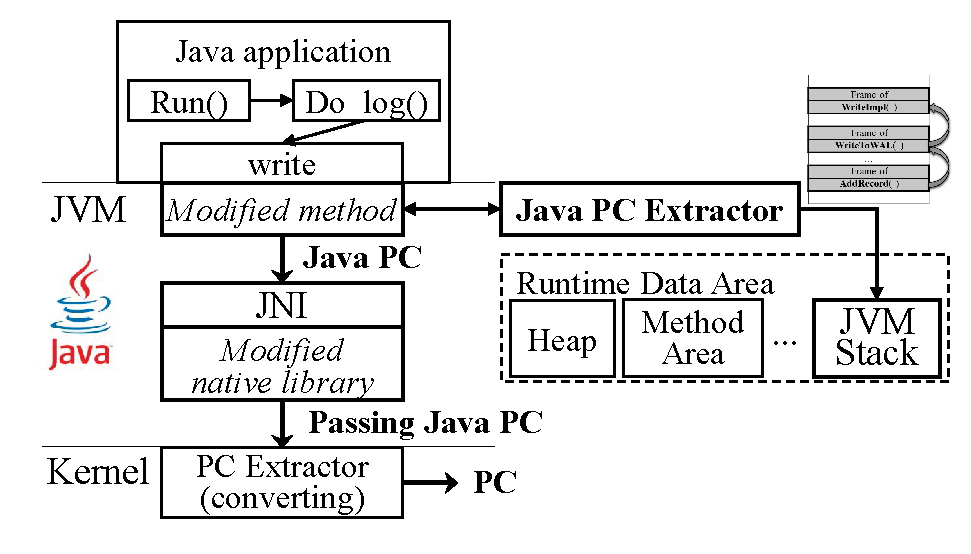
\includegraphics[width=0.6\linewidth]{figure/jvmpc}
\caption{Extracting PCs for JVM}
\label{fig:java}
\end{figure}


\subsection{PC extraction for indirect writes}
One limitation of using PCs to extract I/O characteristics is that it only
works with C/C++ programs that \textit{directly} call write-related system
calls.  Many programs, however, often invoke write system calls
\textit{indirectly} through intermediate layers, which makes it difficult to
track program contexts.

The most representative example may be Java programs, such as Cassandra and
Hadoop, that run inside a Java Virtual Machine (JVM). Java programs invoke
write system calls via a native library written in C, so the PC extractor fails
to capture I/O activities of application logics because it is unable to see the
stack of Java programs.  Another example is C/C++ programs that use a write
buffer dedicated to dealing with writes from application logics. For example,
in MySQL~\cite{MySQL} and PostgreSQL~\cite{PostgreSQL}, all the writes are first
destined for a write buffer, and then flush threads materialize buffered data
to persistent storage later.  In that case, the PC extractor only captures PCs
of flush threads since application logics run in other threads with different
stacks.

The problem of indirect writes can be addressed by collecting PC signatures at
the front-end interface of an intermediate layer that accepts write requests
from application logics. In case of Java programs, a native library can be
modified to capture write requests and computes PC signatures. Once a native
library is modified, it automatically gathers PC signatures without modifying
application code. Fig.~\ref{fig:java} illustrates how \textsf{PCStream}
collects signatures from Java programs.  
We modified the jvm using OpenJDK~\cite{OpenJDK} to extract PC signatures for 
most of write methods in write related classes including \texttt{OutputStream}.
The stack area in \texttt{Runtime Data Areas} of JVM used to calculate PC signatures.
The calculated PC is, then, passed to the write system call of the kernel via
the modified native I/O libraries.

Unlike Java, there is no a straightforward way to support PC collection for
applications with write buffers. This is because the implementation of write
buffering is different depending on applications, so additional efforts are
needed to manually modify code. However, this manual modification is only
limited to a write buffering module, and application logics themselves don't
need to be edited or annotated.



\subsection{\textcolor{red}{TODO: Internal stream management ???}}


%{\color{blue} 추가로, SSD가 지원하는 stream의 개수가 변경되는 상황에서도
%reclustering을 통해
%대응이 가능하다.
%reclustering의 주기는 workload의 변화 패턴에 따라 결정될 수 있다.
%새로운 PC가 계속적으로 생성되거나 한 PC의 수명 패턴이 자주 변화할 경우 reclustering의 주기를 
%좀 더 짧게 설정하여 workload 변화를 반영한다.
%}
%Since the
%number of PCs created by applications is not limited, the clustering algorithm
%must be efficient enough to quickly handle many PCs. 


